\documentclass[varwidth=\maxdimen]{standalone}
\usepackage{tikz}
\usetikzlibrary{fit}
\usepackage[nomessages]{fp}

\tikzset{every label/.style={font=\footnotesize,inner sep=1.5pt}}

\newcommand{\pc}[4][]{\node[circle, fill, label={below:#4},#1] at (#2) (#3) {}}
\newcommand{\pcghost}[4][]{\node[circle, fill=gray, label={below:#4},#1] at (#2) (#3) {}}
\newcommand{\pu}[4][]{\node[rectangle, fill=blue, label={above:#4},#1] at (#2) (#3) {}}
\newcommand{\pughost}[4][]{\node[rectangle, fill=gray, label={above:#4},#1] at (#2) (#3) {}}
\newcommand{\pv}[4][]{\node[rectangle, fill=red, label={below:#4},#1] at (#2) (#3) {}}
\newcommand{\nx}{3} %number of cells in x direction
\newcommand{\ny}{3} %number of cells in y direction
\newcommand{\nghost}{1} %number of ghost cells in x direction
\newcommand{\xmin}{0}  %grid start
\newcommand{\xmax}{12} %grid end
\newcommand{\ymin}{0}  %grid start
\newcommand{\ymax}{12} %grid end

\begin{document}
	\begin{figure}[h]
		\centering
		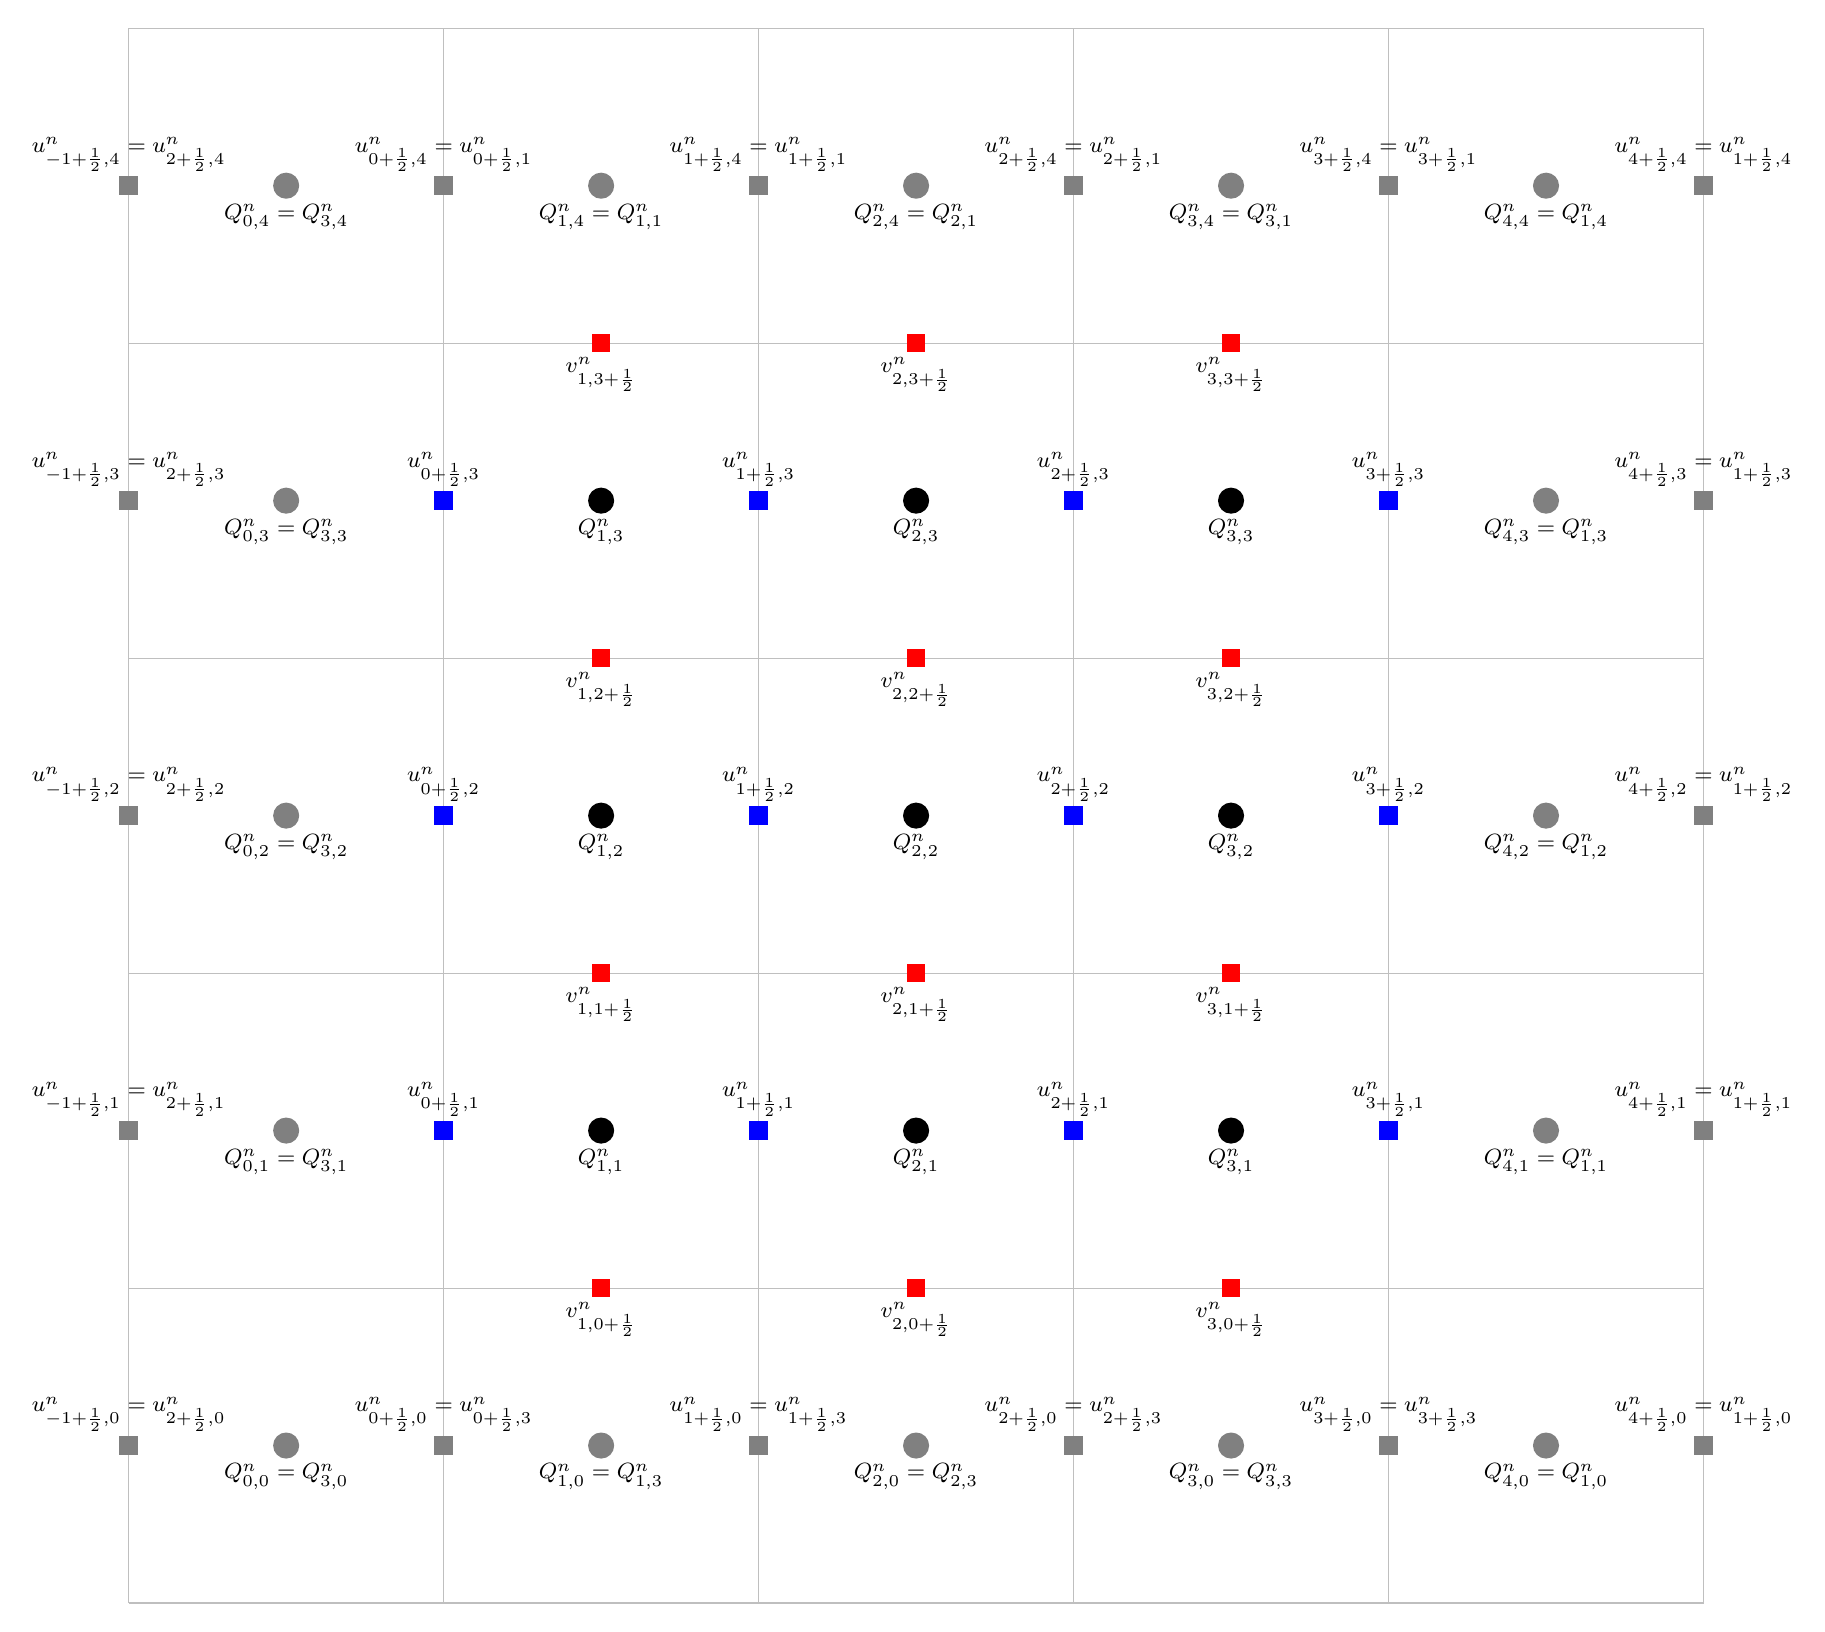
\begin{tikzpicture}
			% Grid lines
			%%%%%%%%%%%%%%%%%%%%%%%%%%%%%%%%%%%%%%%%%%%%%%%%%%%%%%%%%%%%%%%
			\FPeval{\dx}{clip((\xmax-\xmin)/\nx)}
			\FPeval{\dy}{clip((\ymax-\ymin)/\ny)}
			\FPeval{\istart}{clip(-nghost)}
			\FPeval{\iend}{clip(\nx+\nghost)}
			\foreach \i in {\istart,...,\iend}{
				\FPeval{\xp}{clip(\xmin+\i*\dx)}					
				\draw[gray!50, thin] (\xp,\ymin -\nghost*\dy)--(\xp,\ymax+\nghost*\dy);
				\draw[gray!50, thin] (\ymin -\nghost*\dy,\xp)--(\ymax+\nghost*\dy,\xp);
			}

			% Interior grid centers
			\foreach \i in {1,...,\nx}{
				\FPeval{\xp}{clip(\xmin+(\i-0.5)*\dx)}
				\foreach \j in {1,...,\ny}{
					\FPeval{\yp}{clip(\ymin+(\j-0.5)*\dy)}
					\pc{\xp,\yp}{5}{$Q_{\i,\j}^n$};
				}
			}

			% Interior grid edge midpoints
			\foreach \i in {1,...,\nx}{
				\FPeval{\xc}{clip(\xmin+(\i-0.5)*\dx)}
				\foreach \j in {0,...,\ny}{
					\FPeval{\yv}{clip(\ymin+(\j)*\dy)}
					\pv{\xc,\yv}{5}{$v_{\i,\j+\frac{1}{2}}^n$};
					\pu{\yv,\xc}{5}{$u_{\j+\frac{1}{2},\i}^n$};
				}
			}

			% Ghost cell edges
			\FPeval{\jstart}{clip(-nghost+1)}]
			\FPeval{\jend}{clip(nx+nghost)}
			\foreach \i in {1,...,\nghost}{
				\foreach \j in {\jstart,...,\jend}{
					\FPeval{\xc}{clip(\xmin-\i*\dx)}
					\FPeval{\yc}{clip(\ymin+(\j-0.5)*\dy)}
					\FPeval{\ii}{clip(\nghost-1-\i)}
					\FPeval{\iii}{clip(\nx-\i)}
				    \pughost{\xc,\yc}{5}{$u_{\ii+\frac{1}{2},\j}^n = u_{\iii+\frac{1}{2},\j}^n$};

					\FPeval{\xc}{clip(\xmax+\i*\dx)}
					\FPeval{\yc}{clip(\ymin+(\j-0.5)*\dy)}
					\FPeval{\ii}{clip(\nx+\i)}
					\FPeval{\iii}{clip(\i)}
					\pughost{\xc,\yc}{5}{$u_{\ii+\frac{1}{2},\j}^n =u_{\iii+\frac{1}{2},\j}^n$};

					\FPeval{\xc}{clip(\xmin-\i*\dx)}
					\FPeval{\yc}{clip(\ymin+(\j-0.5)*\dy)}
					\FPeval{\ii}{clip(\nghost-1-\i)}
					\FPeval{\iii}{clip(\nx-\i)}
					%\pughost{\yc,\xc}{5}{$v_{\j,\ii+\frac{1}{2}}^n = %v_{\j,\iii+\frac{1}{2}}^n$};

					\FPeval{\xc}{clip(\xmax+\i*\dx)}
					\FPeval{\yc}{clip(\ymin+(\j-0.5)*\dy)}
					\FPeval{\ii}{clip(\nx+\i)}
					\FPeval{\iii}{clip(\i)}
					%\pughost{\yc,\xc}{5}{$v_{\j,\ii+\frac{1}{2}}^n =v_{\j,\iii+\frac{1}{2}}^n$};
				}
			}

			% Ghost cell edges
			\foreach \j in {1,...,\nghost}{
				\foreach \i in {0,...,\nx}{
					\FPeval{\xc}{clip(\xmin+\i*\dx)}
					\FPeval{\yc}{clip(\ymax+(\j-0.5)*\dy)}
					\FPeval{\jj}{clip(\j+\ny)}
					\FPeval{\jjj}{clip(\j)}
					\pughost{\xc,\yc}{5}{$u_{\i+\frac{1}{2},\jj}^n = u_{\i+\frac{1}{2},\jjj}^n$};

					\FPeval{\xc}{clip(\xmin+\i*\dx)}
					\FPeval{\yc}{clip(\ymin-(\j-0.5)*\dy)}
					\FPeval{\jj}{clip(\j-1)}
					\FPeval{\jjj}{clip(\ny+1-\j)}
					\pughost{\xc,\yc}{5}{$u_{\i+\frac{1}{2},\jj}^n = u_{\i+\frac{1}{2},\jjj}^n$};

					\FPeval{\xc}{clip(\xmin+\i*\dx)}
					\FPeval{\yc}{clip(\ymax+(\j-0.5)*\dy)}
					\FPeval{\jj}{clip(\j+\ny)}
					\FPeval{\jjj}{clip(\j)}
					%\pughost{\yc,\xc}{5}{$v_{\i+\frac{1}{2},\jj}^n = v_{\i+\frac{1}{2},\jjj}^n$};

					\FPeval{\xc}{clip(\xmin+\i*\dx)}
					\FPeval{\yc}{clip(\ymin-(\j-0.5)*\dy)}
					\FPeval{\jj}{clip(\j+\ny)}
					\FPeval{\jjj}{clip(nx+1-\j)}
					%\pughost{\yc,\xc}{5}{$v_{\jj,\i+\frac{1}{2}}^n = v_{\jjj,\i+\frac{1}{2}}^n$};
				}
			}

			% Ghost cell centers
			\FPeval{\jstart}{clip(-nghost+2)}]
			\FPeval{\jend}{clip(nx+nghost+1)}
			\foreach \i in {1,...,\nghost}{
				\foreach \j in {\jstart,...,\jend}{
					\FPeval{\xc}{clip(\xmin-(\nghost-\i+0.5)*\dx)}
					\FPeval{\yc}{clip(\ymin-(\nghost-\j+0.5)*\dx)}
					\FPeval{\ii}{clip(\i-\nghost)}
					\FPeval{\iii}{clip(\nx+\ii)}
					\FPeval{\jj}{clip(\j-1)}
					\pcghost{\xc,\yc}{5}{$Q_{\ii,\jj}^n=Q_{\iii,\jj}^n$};

					\FPeval{\xc}{clip(\xmax+(\i-0.5)*\dx)}
					\FPeval{\ii}{clip(\nx+\i)}
					\FPeval{\iii}{clip(\i)}
					\FPeval{\jj}{clip(\j-1)}
					\pcghost{\xc,\yc}{5}{$Q_{\ii,\jj}^n=Q_{\iii,\jj}^n$};
				}
			}


			% Ghost cell centers
			\FPeval{\jstart}{clip(-nghost+1)}]
			 \foreach \i in {1,...,\nx}{
				\foreach \j in {1,...,\nghost}{
					\FPeval{\xc}{clip(\xmin+(\i-0.5)*\dx)}
					\FPeval{\yc}{clip(\ymin-(\j-0.5)*\dx)}
					\FPeval{\jjj}{clip(\nx-1+\j)}
					\FPeval{\jj}{clip(\j-1)}
					\pcghost{\xc,\yc}{5}{$Q_{\i,\jj}^n=Q_{\i,\jjj}^n$};
		
					\FPeval{\yc}{clip(\ymax+(\j-0.5)*\dx)}
					\FPeval{\jjj}{clip(\j)}
					\FPeval{\jj}{clip(nx+\j)}
					\pcghost{\xc,\yc}{5}{$Q_{\i,\jj}^n=Q_{\i,\jjj}^n$};
				}
			}
		\end{tikzpicture}
	\end{figure}
\end{document}
